\chapter{Item2Vector Neural Network Architecture}
\label{cha:1}
The success of Neural network models especially the Word2Vector model has been a great inspiration for this Item2Vector model. We see that the distributed vector representation of words has been so powerful in capturing a lot of local information which many other algorithms like Latent Semantic Indexing are not able to capture. One of the most important objectives of this thesis is to similarly develop a \textbf{distributed representation of items} in the corpus so that each user can be represented as a linear combination of the items that he has rated. Thereafter a collaborative filtering based recommendation system can be built in this low-dimensional space.  We accomplish the objective of developing a distributed representation of items in the corpus with a simple two layer Neural network very similar to Word2Vector model which we shall name as Item2Vector model (named after its inspiration). This chapter has the following sections:
\begin{myitemize}
    \item Architecture of the Item2Vector Neural Network
    \begin{myitemize}
        \item Input, Output, Activation Function
    \end{myitemize}
    \item Forward Propagation Algorithm
    \item Loss functions
    \item Parameter Learning
    \begin{myitemize}
         \item Backpropagation Algorithm
        \item Stochastic Gradient descent Algorithm
    \end{myitemize}
\end{myitemize}


We start this chapter by reasoning out the inspiration of this model to the reader, and then introducing the architecture of the Item2Vector Neural network, followed by a discussion of the Forward Propagation algorithm in which the input is propagated  across the hidden layer and the output is estimated.  Later on, we discuss the possible different loss/objective functions which estimates the efficiency of our model. Following this, we discuss the back propagation algorithm and the stochastic gradient descent algorithm to optimize the parameters of the model, consequently optimizing the cost function. 

\section{Reasoning out the inspiration}


\section{Description of the Neural Network Architecture}
\begin{figure}
  \centering
  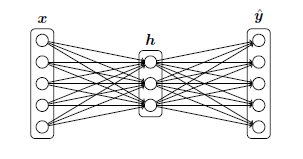
\includegraphics{2_1_NN_Architecture}
  \caption{A Simple Item2Vector Neural Network Architecture}
  \label{fig:2_1_NN_Architecture}
\end{figure}

\fref{fig:2_1_NN_Architecture} The Item2Vector Neural Network is fully connected two layer Neural Network (One hidden layer and one output layer). The size of the hidden layer i.e. the number of hidden neurons, depends upon the data set and the type of application. In general it is preferable to choose the size of the hidden layer using cross validation if regularization parameters have not been employed. In our case the size of the hidden layer is equal to the number of Eigen vectors retained while building the SVD model so that we can have a fair comparison at the end.



\begin{center}
[Twilight Part 1, Twilight Part 2, Twilight Part 3, Twilight Part 4, Twilight Part 5]
\end{center}

In case of Skip-gram model, when an item is given as input called as center item, all the items which usually occur along with it called as co-occuring items are predicted. For example, when Twilight Part 2 is given as input, the co-occuring items Twilight Part 1, 3, 4 and 5 are predicted as output. 

In the case of a CBOW model the reverse is true. For example when Twilight Part 1, 2, 3, 4 are given as input, Twilight Part 5 is predicted. 

\subsection{Input to the Neural Network}
The list of items present in the corpus is referred to as the item list. The input to the Neural network is a one hot encoded vector. The one hot encoding depends on the type of the model employed for generating the Item Vectors. In case of the Skip-gram model, the index of the center item is one-hot encoded in the item list and given as input. Whereas in the case of CBOW model, the indices of the co-occuring items is one-hot encoded and given as input. 

\subsection{Hidden Layer and Activation Function}
Let $\boldsymbol{}$ be the one-hot encoded input vector and $\boldsymbol{W_1}$ and $\boldsymbol{b_1}$ be the matrix of weights and vector of biases connecting the input layer to the hidden layer. In the beginning the weights and biases are initialized to some small random values. During the forward propagation, the hidden layer gets initialized as shown in \ref{eqn:ForwardProp_1} :

\begin{equation} \label{eqn:ForwardProp_1}
h=sigmoid(x W_1+b1)
\end{equation}

\subsection{Output layer and Softmax Function}
Let \^{y} be the output vector and $\boldsymbol{W_2}$ and $\boldsymbol{b_2}$ be the matrix of weights and vector of biases connecting the hidden layer to the output layer. The Output vector is estimated as shown in \ref{eqn:ForwardProp_2}:

\begin{equation} \label{eqn:ForwardProp_2}
\hat{y}=softmax(h W_2+b2)
\end{equation}

\section{Adding more intuitive insight to the Neural Network Architecture}
The Skip-gram model as well as the CBOW model results in two vectors corresponding to each item in the list of items. These vectors are called as input and output vectors. The sigmoid of Weights $W_1$ + bias $b_1$ connecting the input layer and the hidden layer, corresponds to the input vector of each item in the list of items. Similarly the weights $W_2$ summed with the bias $b_2$ connecting the hidden layer and the output layer corresponds to the output vector of each item in the list of items. 

After the training, the sigmoid of the sum of vector of weights from an input neuron to each hidden neuron and the bias is the input vector of the item. 
\begin{center}
$v_i=sigmoid(W_{1i}+b1)$
\end{center}
Here, $v_i$ is the input vector of the $i^{th}$ item. 

Similarly the sum of the vector of the weights from all the hidden neurons to one output neuron corresponds to the output vector of that item.
\begin{center}
$u_i=W_{2i}+b2$
\end{center}

Here, $u_i$ is the input vector of the $i^{th}$ item. 

In case of a Skip-gram model, we want to predict the probability of an item co-occuring with an other item. Therefore the similarity of the input vector of the given item and the output vector of the other item is estimated using a simple dot product and then crunched into probability using a soft-max function.

\begin{equation}
\hat{y_{ij}}=softmax(v_i*u_j)
\end{equation}
Here $\hat{y_{i,j}}$ refers to the probability of the $i^{th}$ item co-occuring with the  $j^{th}$ item.

\section{Training the Neural Network}
Let our Neural Network consists of $nh$ hidden neurons, $D_x$ input neurons each corresponding to one item in the list of items and $D_y$ output neurons each corresponding to one item in the list of items. It can been seen that $D_x=D_y$. Therefore our Neural Network consists of $(D_x+1)*nh + (nh+1)*D_y$ parameters.

\subsection{Loss Functions}
I evaluated the performance of the model while optimizing two types of loss functions. The first one is the cross entropy loss and the second one is negative sampling. 
\subsubsection{Cross Entropy Loss}
Cross entropy loss can be estimated as shown in \ref{eqn:Cross_Entropy}

\begin{equation}
J_{CE}(y,\hat{y})=\sum_{i}^{D_y}y_i log(\hat{y_i})
\label{eqn:Cross_Entropy}
\end{equation}

\begin{equation}
\hat{y_i}=p(i|c)=\frac{exp(u_i^T v_c )}{\sum_{w=1}^{D_y}u_w^T v_c}
\label{y_hat}
\end{equation}

\subsubsection{Negative Sampling Loss Function}
The Negative sampling loss function can be estimated as shown in \ref{eqn:Negative_loss}

\begin{equation}
J_{neg-sample}=-log(\sigma(u_o^T v_c))-\sum_{k=1}^{K} log (-\sigma(u_k^T v_c))
\label{eqn:Negative_loss}
\end{equation}





%%% Local Variables: 
%%% mode: latex
%%% TeX-master: "thesis"
%%% End: 
